%&latexf
\documentclass[a4paper]{article}
\usepackage{color}
\setlength{\hoffset}{-0.5in}\hoffset-0.5in
\setlength{\textwidth}{15cm}
\usepackage{hyperref}
\usepackage{amsmath, amsfonts, amsthm, amssymb}
\usepackage{verbatim}
\usepackage{stmaryrd}
\usepackage{fancyhdr}
\usepackage{color}
\usepackage[dvips]{graphicx}
\usepackage{subfigure}
\linespread{1.5}
%\font\twelvemsb=msbm10 at 12pt
\newfam\msbfam
%\textfont\msbfam=\twelvemsb
\def\Bbb#1{\fam\msbfam\relax#1}

\topmargin = 20pt
\voffset = -20pt
\addtolength{\textheight}{2cm}
\newtheorem{theorem}{Theorem}[section]
\newtheorem{exa}{Example}[section]
\newtheorem{corollary}[theorem]{Corollary}
\newtheorem{lemma}[theorem]{Lemma}
\newtheorem{proposition}[theorem]{Proposition}

\theoremstyle{definition}
\newtheorem{definition}[theorem]{Definition}
\newtheorem{remark}[theorem]{Remark}
\newtheorem{notation}[theorem]{Notation}
\newtheorem{assumption}[theorem]{Assumption}
\newtheorem{conjecture}[theorem]{Conjecture}

\newcommand{\ind}{1\hspace{-2.1mm}{1}} %Indicator Function
\newcommand{\I}{\mathtt{i}}
\newcommand{\D}{\mathrm{d}}
\newcommand{\E}{\mathrm{e}}
\newcommand{\RR}{\mathbb{R}}
\newcommand{\sgn}{\mathrm{sgn}}
\newcommand{\atanh}{\mathrm{arctanh}}
\def\equalDistrib{\,{\buildrel \Delta \over =}\,}
\numberwithin{equation}{section}
\def\blue#1{\textcolor{blue}{#1}}
\def\red#1{\textcolor{red}{#1}}


\begin{document}

\thispagestyle{empty}
\null\vskip0.2in%
\begin{center}
\LARGE{{\bf 
TITLE OF THE THESIS}}
\end{center}

\vspace{0.5cm}

\begin{center}
{\Large {\bf by}}\\
\mbox{} \\
{\Large {\bf Author (CID: ...)}}
\end{center}

\vspace{1cm}

\begin{center}
\large{\bf{Department of Mathematics \\ Imperial College London \\
London SW7 2AZ \\ United Kingdom}}
\end{center}


\vspace{1.5cm}

\begin{figure}[!h]
\centering

\includegraphics[scale=0.4]{IC_Crest.eps}
\end{figure}

\vspace{1.5cm}

\begin{center}
\large{\bf{Thesis submitted as part of the requirements for the award of the \\
MSc in Mathematics and Finance, Imperial College London, 2012-2013}}
\end{center}

\vspace{2cm}


%\thispagestyle{empty}

\mbox{}\newline\vspace{10mm} \mbox{}\LARGE
%
{\bf Acknowledgements} \normalsize \vspace{5mm}

I would like to thnk my supervisor.....
%%%%%%%%%%%%%%%%%%%%%%%%%%%%%%%%%%%%%%%%%%%%%%%%%%%%
%\text{}\newpage
%%%%%%%%%%%%%%%%%%%%%%%%%%%%%%%%%%%%%%%%%%%%%%%%%%%%
\setcounter{tocdepth}{4}
\tableofcontents
\newpage
%\newpage
%\include{ThesisNotations}
%%%%%%%%%%%%%%%%%%%%%%%%%%%%%%%%%%%%%%%%%%%%%%%%%%%%
\fancyhead{}
\fancyfoot{}
\pagestyle{fancy} 
%\fancyhead{\sffamily\small \thepage}
%\fancyhead{\sffamily\small \nouppercase{\rightmark}}
\fancyhead[RO,LE]{\sffamily\small \thepage}
\fancyhead[LO,RE]{\sffamily\small \nouppercase{\rightmark}}
\renewcommand{\headrulewidth}{0.4pt}
\renewcommand{\footrulewidth}{0.0pt}
%%%%%%%%%%%%%%%%%%%%%%%%%%%%%%%%%%%%%%%%%%%%%%%%%%%%
%\include{Thesis_Part1_Introduction}
%\include{Thesis_Part2_Tools}
%\include{Thesis_Part3_Large}
%\include{Thesis_Part4_Small}




%%%%%%%%%%%%%%%%%%%%%%%%%%%%%%%%%%%%%%%%%%%%%%%%%%%%
\section{Introduction}
General introduction.

%%%%%%%%%%%%%%%%%%%%%%%%%%%%%%%%%%%%%%%%%%%%%%%%%%%%
\section{Option pricing}
\subsection{The fundamental theorem of asset pricing}

\subsection{The Black-Scholes model}
Consider a given probability space $(\Omega, (\mathcal{F})_t,\mathbb{P})$ 
supporting a Brownian motion~$(W_t)_{t\geq 0}$.
In the Black-Scholes model, the stock price process~$(S_t)_{t\geq 0}$ is the unique strong solution to
the following stochastic differential equation:
\begin{equation}\label{eq:BS}
\frac{\D S_t}{S_t} = r \D t + \sigma \D W_t,
\qquad S_0>0,
\end{equation}
where $r\geq 0$ denotes the instantaneous risk-free interest rate and $\sigma>0$ the instantaneous volatility.

\subsubsection{No interest rates}
\subsubsection{Including interest rates}
A European call price $C_t(S_0,K,\sigma)$ with maturity $t>0$ and strike $K>0$ 
pays at maturity $(S_t-K)_+=\max(S_t-K,0)$. 
When the stock price follows the Black-Scholes SDE~\eqref{eq:BS}, 
Black and Scholes~\cite{BS73} proved that its price at inception is worth
$$
C_t(S_0,K,\sigma) = S_0\mathcal{N}(d_+) - K\E^{-rt}\mathcal{N}(d_-),
$$
where
$$
d_{\pm} := \frac{\log\left(S_0 \E^{rt}/K\right)}{\sigma\sqrt{t}} \pm \frac{\sigma\sqrt{t}}{2},
$$
and where~$\mathcal{N}$ denotes the cumulative distribution function of the Gaussian random variable.

Here is an example of how to insert a picture:

\begin{figure}[!ht]
\centering
\subfigure{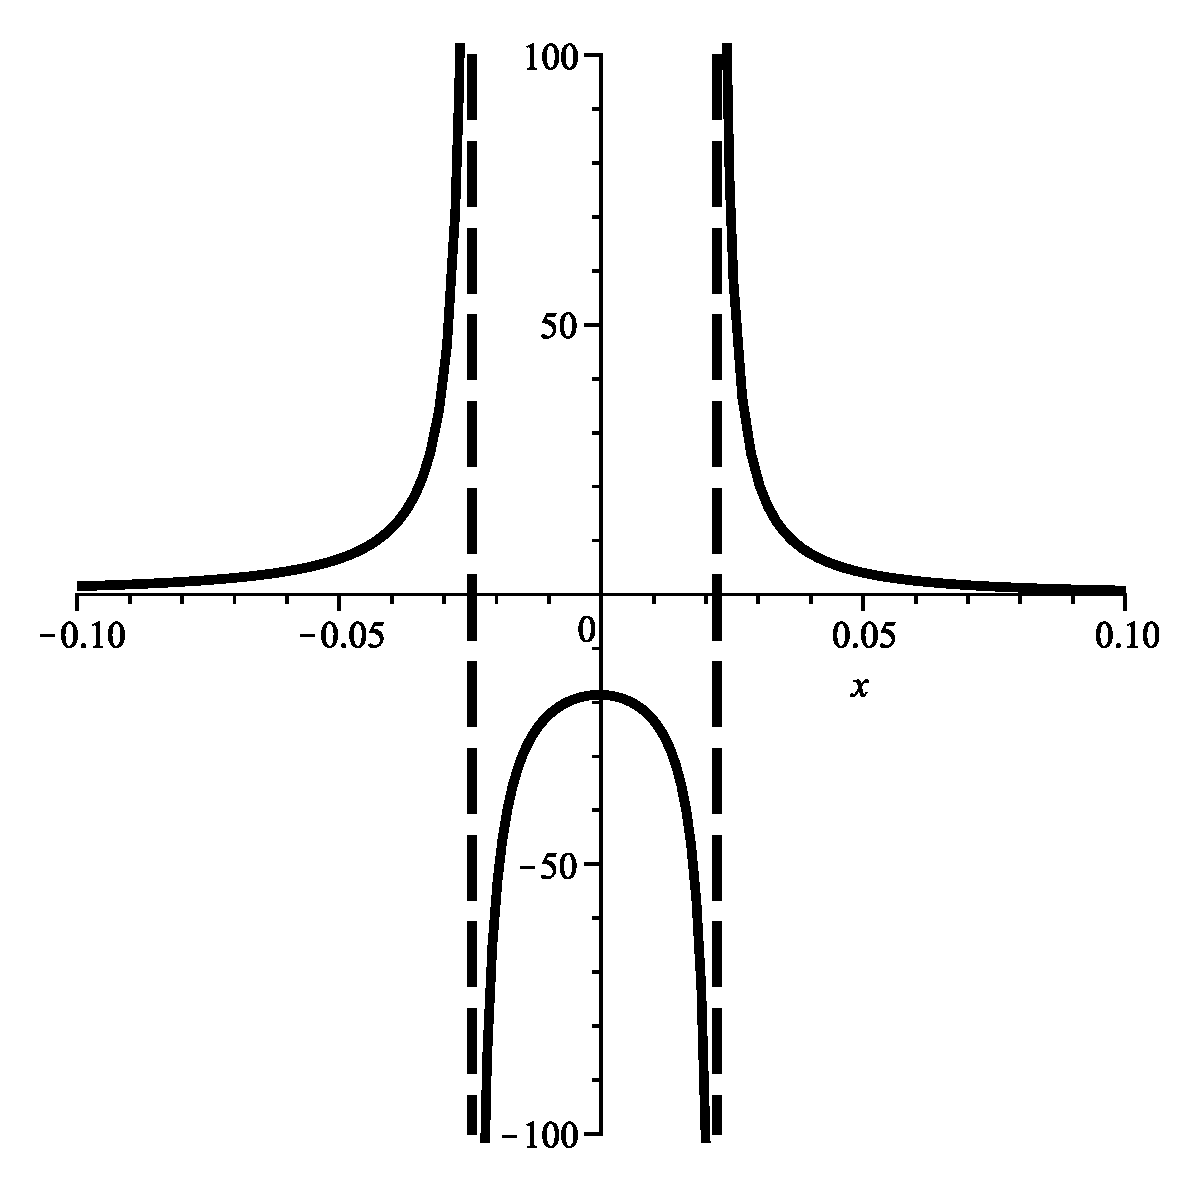
\includegraphics[scale=0.2]{Picture.eps}}
\caption{This is the caption for the figure.}
\label{fig:Pict}
\end{figure}

or two side-by-side pictures:

\begin{figure}[!ht]
\centering
\subfigure{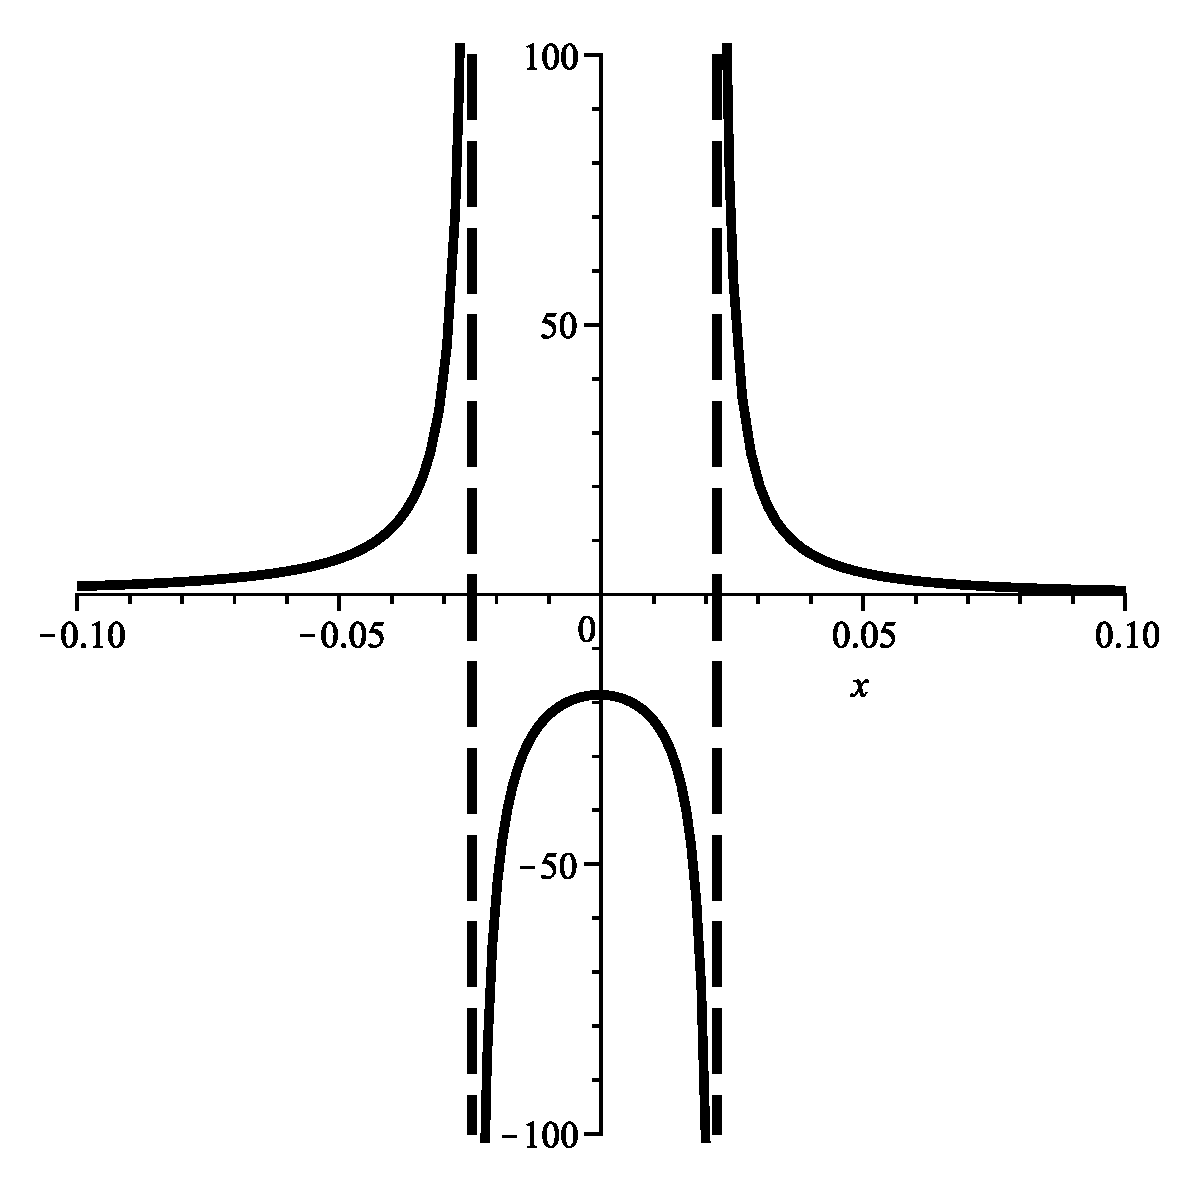
\includegraphics[scale=0.3]{Picture.eps}}
\hspace{15pt}
\subfigure{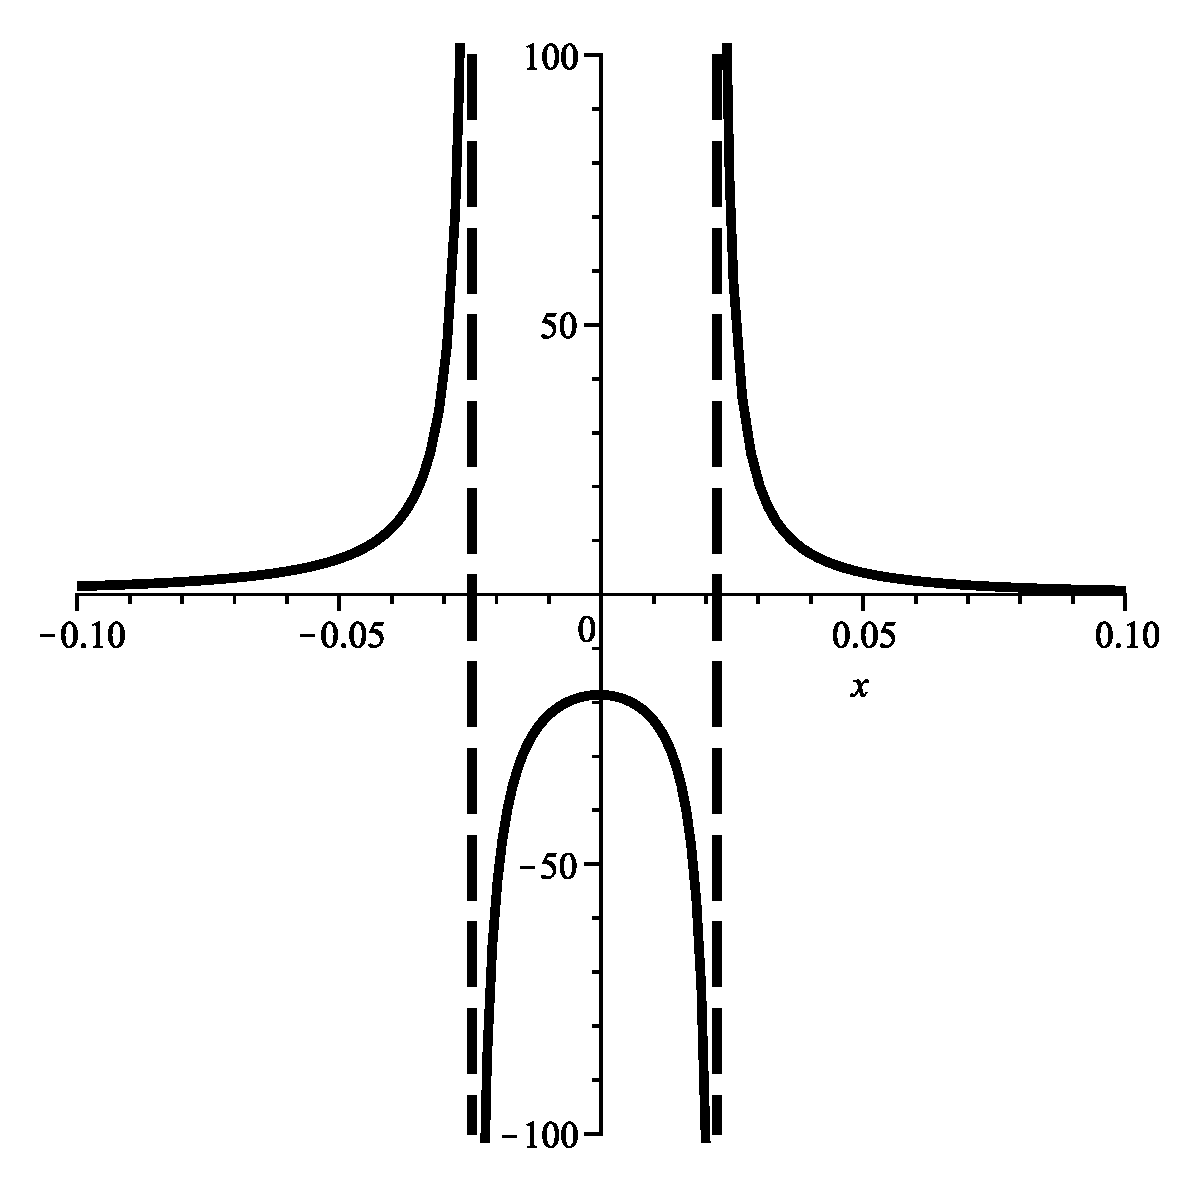
\includegraphics[scale=0.3]{Picture.eps}}
\caption{Blablabla}
\label{fig:Pict2}
\end{figure}


\newpage
%%%%%%%%%%%%%%%%%%%%%%%%%%%%%%%%%%%%%%%%%%%%%%%%%%%%
%%%%%%%%%%%%%%%%%%%%%%%%%%%%%%%%%%%%%%%%%%%%%%%%%%%%
\section{Model calibration}
\subsection{What is calibration?}
Here is an example of a matrix in $A\in\mathcal{M}_n(\RR)$:
$$
A = 
\begin{pmatrix}
a_{11} & a_{12} & \ldots & a_{1n}\\
a_{21} & \ddots & \ddots  & \vdots\\
\vdots &  \ddots & \ddots  & \vdots\\
a_{n1} &  \ldots &  \ldots & a_{1n}.
\end{pmatrix}
$$

\subsection{Numerical methods for calibration}
...




%%%%%%%%%%%%%%%%%%%%%%%%%%%%%%%%%%%%%%%%%%%%%%%%%%%%
%%%%%%%%%%%%%%%%%%%%%%%%%%%%%%%%%%%%%%%%%%%%%%%%%%%%
\appendix

\section{Review of stochastic calculus}
\subsection{Riemann integration}
\subsection{The It\^o integral}


\section{Some technical proofs}



%%%%%%%%%%%%%%%%%%%%%%%%%%%%%%%%%%%%%%%%%%%%%%%%%%%%
%%%%%%%%%%%%%%%%%%%%%%%%%%%%%%%%%%%%%%%%%%%%%%%%%%%%
\newpage
\addcontentsline{toc}{part}{\protect\numberline{}Conclusion}
\vspace{1.5cm}
\begin{center}
\Huge{{\bf Conclusion}}
\end{center}
\vspace{0.5cm}
Conclusion if needed...

%%%%%%%%%%%%%%%%%%%%%%%%%%%%%%%%%%%%%%%%%%%%%%%%%%%%
%%%%%%%%%%%%%%%%%%%%%%%%%%%%%%%%%%%%%%%%%%%%%%%%%%%%
\begin{thebibliography}{9}
\bibitem{BS73}F.~ Black and M.~Scholes.
The Pricing of Options and Corporate Liabilities.
\textit{Journal of Political Economy}, {\tt 81} (3): 637-659, 1973.

\bibitem{KS97}I.~ Karatzas and S.E.~Shreve.
Brownian Motion and Stochastic Calculus.
Springer-Verlag, 1997.

\bibitem{KT81}S.~Karlin and H.~Taylor.
A Second Course in Stochastic Processes. 
Academic Press, 1981.

\bibitem{Tank} P.~Tankov.
Pricing and hedging in exponential L\'evy models: review of recent results. 
\textit{Paris-Princeton Lecture Notes in Mathematical Finance}, Springer, 2010. 

\bibitem{W03}D.~Williams.
Probability With Martingales.
CUP, 1991.

\end{thebibliography}


\end{document}
